\chapter{Champ électrique}

\section{Qu'est-ce que le champ électrique?}

\marginpar{Tremblay \S 2.1}


\paragraph{Objectif}
\begin{enumerate}
  \item L'étudiante comprendra ce qu'est un champ électrique.
  \item Elle pourra calculer le champ électrique produit par un ensemble de
    charges ponctuelles en appliquant le principe de superposition.
\end{enumerate}


\marginpar{5 minutes}
  Le concept d'action à distance est troublant. La loi de Coulomb suggère que
  si deux charges interagissent et que l'une des deux se déplace, l'autre
  subira les effets instantanément. Or, cela voudrait dire qu'il est possible
  de faire voyager de l'information plus vite que la vitesse de la lumière. De
  plus, des expériences minutieuses confirment qu'il y a un délai avant que la
  deuxième charge ne détecte un changement de la position de la première. Ce
  délai est de l'ordre de \SI{1e-8}{s} pour deux charges séparées d'environ
  \SI{1}{m}.

  Il faut donc un intermédiaire entre les deux charges. Cet intermédiaire est
  le \textbf{champ électrique}. Un objet chargé génère autour de lui un
  champ électrique.


\subsection*{Analogie avec le champ gravitationnel}
\marginpar{5 minutes}

Selon la loi de la gravitation universelle de Newton
\[
  F_g = \frac{Gm_1m_2}{r^2}.
\]
La partie $Gm_1 / r^2$ ne dépend que de la source du champ gravitationnel et de
la distance entre le centre de masse de cet objet et le point où on veut
calculer la force. Par exemple, à la surface de la Terre on a
\[
  \frac{GM_\oplus}{R_\oplus^2} = \SI{9.8}{m/s^2} \equiv g
\]
et on peut calculer la force sur un objet de masse $m$ à la surface de la Terre
avec
\[
  F_g = mg.
\]
Pour la force électrique, c'est le même principe. À partir de la loi de
Coulomb
\[
  F_e = \frac{k\abs{q_1}\abs{q_2}}{r^2}
\]
on reconnait qu'une partie de l'expression ne dépend que de la source et de la
distance à laquelle on se trouve de cette source
\[
  E = \frac{k\abs{q_1}}{r^2}.
\]
On peut calculer la force sur une particule chargée située à une distance $r$
de $q_1$ en faisant simplement
\[
  F_e = E\abs{q_2}.
\]




\section{Champ électrique d'une charge ponctuelle}
\marginpar{Tremblay \S 2.2}

\marginpar{5 minutes}

  $$\vec{E} = \frac{kq}{r^2} \vec{u}_{r}$$

  où $\vec{u}_r$ est un vecteur unitaire qui s'éloigne de la charge ponctuelle.

  \begin{center}
  \begin{tikzpicture}
    \matrix[column sep=1.5cm] {
    \node[positive, circle] (q) at (0, 0) {$+$};
    \foreach \theta in {0, 30, ..., 330} {
      \draw[->] (q) -- ++(\theta:1);
      \draw[->] ($(q) + (\theta:1.05)$) -- ++(\theta:0.5);
      \draw[->] ($(q) + (\theta:1.05) + (\theta:0.55)$) -- ++(\theta:0.25);
    }
    &
    \node[negative, circle] at (0, 0) {$-$};
    \foreach \theta in {0, 30, ..., 330} {
      \draw[<-] (q) -- ++(\theta:1);
      \draw[<-] ($(q) + (\theta:1.05)$) -- ++(\theta:0.5);
      \draw[<-] ($(q) + (\theta:1.05) + (\theta:0.55)$) -- ++(\theta:0.25);
    }
    \\
    };
  \end{tikzpicture}
  \end{center}



\subsection*{Exercice}
\marginpar{5 minutes}
\marginpar{Diapo}
  Dans chacune des situations ci-dessous, utilisez les informations fournies
  pour trouver la direction du champ électrique à la position de la charge de
  droite.

  \begin{enumerate}
    \item
      \begin{tikzpicture}
        \node[positive, circle] (q1) at (0, 0) {$+$};
        \node[positive, circle] (q2) at (2, 0) {$+$};
      \end{tikzpicture}
    \item
      \begin{tikzpicture}
        \node[positive, circle] (q1) at (0, 0) {$+$};
        \node[negative, circle] (q2) at (2, 0) {$-$};
      \end{tikzpicture}
    \item
      \begin{tikzpicture}
        \node[negative, circle] (q1) at (0, 0) {$-$};
        \node[positive, circle] (q2) at (2, 0) {$+$};
      \end{tikzpicture}
    \item
      \begin{tikzpicture}
        \node[draw, circle] (q1) at (0, 0) {$q$};
        \node[negative, circle] (q2) at (2, 0) {$-$};
        \draw[very thick, ->] (q2) -- ++(1.5, 0) node[right] {$\vec{F}$};
      \end{tikzpicture}
    \item
      \begin{tikzpicture}
        \node[positive, circle] (q1) at (0, 0) {$+$};
        \node[draw, circle] (q2) at (2, 0) {$q$};
        \draw[very thick, ->] (q2) -- ++(-1.5, 0) node[below] {$\vec{F}$};
      \end{tikzpicture}
  \end{enumerate}


\subsection*{Principe de superposition}
\marginpar{5 minutes}

  Le champ électrique total en un point de l'espace est la somme des champs
  électrique causés par toutes les charges à proximité.

  On peut voir que c'est vrai à partir du principe de superposition pour les
  forces électriques.
  \begin{eqnarray*}
    \vF = q\vec{E} &=& \vF_1 + \vF_2 + \cdots + \vF_n \\
          &=& q \vec{E}_1 + q \vec{E}_2 + \cdots + q \vec{E}_n \\
          &=& q \left( \vec{E}_1 + \vec{E}_2 + \cdots + \vec{E}_n \right)
  \end{eqnarray*}



\subsection*{Exercice}
\marginpar{25 minutes}
  Une charge $q = \SI{30}{\micro\coulomb}$ est placée à \SI{160}{cm} du sol. À
  droite de cette charge, une charge $Q = \SI{-50}{\micro\coulomb}$ est placée
  à \SI{2}{m} au-dessus du sol. La distance entre les deux charges est $D =
  \SI{3}{m}$.

  Calculer le champ électrique au point $P$ situé à \SI{1}{m} à droite de la
  charge $q$ et à \SI{4}{m} au-dessus du sol.

  \begin{center}
    \includegraphics[scale=0.25]{02-champ-electrique/figures/champ-deux-charges-1.pdf}
  \end{center}

  \sectionline

\paragraph{Solution}
  Les coordonnées du point $P$ sont $x = \SI{1}{m}$, $y = \SI{2.4}{m}$.
  \begin{center}
    \includegraphics[scale=0.5]{02-champ-electrique/figures/champ-deux-charges-soln.pdf}
  \end{center}
  Le champ électrique de la charge $q$ au point $P$ est de grandeur et
  composantes
  \begin{align*}
    E_q &= \frac{k\abs{q}}{x^2 + y^2} \\
    E_{qx} &= E_q \cos \theta
        &= \frac{k\abs{q}}{x^2 + y^2} \frac{x}{\sqrt{x^2 + y^2}}
        &= \frac{k\abs{q}x}{(x^2 + y^2)^{3/2}}
        &= \SI{15344}{N/C} \\
    E_{qy} &= E_q \sin \theta
        &= \frac{k\abs{q}}{x^2 + y^2} \frac{y}{\sqrt{x^2 + y^2}}
        &= \frac{k\abs{q}y}{(x^2 + y^2)^{3/2}}
        &= \SI{36827}{N/C} \\
  \end{align*}
  Le champ électrique de la charge $Q$ au point $P$ est de grandeur et
  composantes
  \begin{align*}
    E_Q &= \frac{k\abs{Q}}{r_Q^2} \\
    E_{Qx} &= E_Q \cos \alpha
        &= \frac{k\abs{Q}}{r_Q^2} \frac{1}{\sqrt{2}}
        &= \frac{k\abs{Q}}{\sqrt{2}r_Q^2}
        &= \SI{39730}{N/C} \\
    E_{Qy} &= -E_Q \sin \alpha
        &= -\frac{k\abs{Q}}{r_Q^2} \frac{1}{\sqrt{2}}
        &= -\frac{k\abs{Q}}{\sqrt{2}r_Q^2}
        &= \SI{-39730}{N/C} \\
  \end{align*}
  Par le principe de superposition
  \begin{align*}
    \vE &= \vE_q + \vE_Q  \\
        &= \left(\num{55075}\xhat - \num{2903}\yhat\right) \si{N/C}
  \end{align*}



\section{Lignes de champ électrique}
\marginpar{Tremblay \S 2.4}

\paragraph{Objectif}

\begin{enumerate}
  \item L'étudiante connaîtra le lien entre les lignes de champ et le champ
    électrique.
  \item L'étudiante pourra utiliser la notion de champ électrique pour calculer
    la force sur une particule chargée.
\end{enumerate}

\paragraph{Démonstration}
\marginpar{10 minutes}

  Matériel
  \begin{enumerate}
    \item Un vase de Pétri
    \item Huile végétale
    \item Graines de gazon
    \item Source de champ électrique (générateur de Van de Graaff)
    \item Électrodes
    \item Fils
  \end{enumerate}

  Manipulations
  \begin{enumerate}
    \item Mettre de l'huile dans le vase de Pétri
    \item Ajouter les graines de gazon dans l'huile
    \item Connecter un fil à la sphère et un fil à la mise à la terre
    \item Connecter l'autre extrémité des fils aux électrodes
    \item Mettre les électrodes dans l'huile et démarrer le Van de Graaf.
  \end{enumerate}


\subsection*{Caractéristiques des lignes de champ}
\marginpar{10 minutes}

  Les lignes de champ électrique permettent de visualiser le champ électrique.
  Lorsqu'on les trace, on doit respecter les règles suivantes :

  \begin{itemize}
    \item le champ électrique est tangent aux lignes de champ;
    \item la norme du champ électrique est proportionnelles à la densité de
      lignes de champ.
    \item les lignes de champ commence sur les charges positives ou à l'infini
    \item les lignes de champ se termine sur les charges négatives ou à
      l'infini
  \end{itemize}

  \begin{center}
      \includegraphics[scale=0.3]{figures/lignes-champ-dipole.pdf}
      \includegraphics[scale=0.3]{figures/lignes-champ-deux-plus.pdf}
  \end{center}

  Conséquences de ces règles :

  \begin{itemize}
    \item le nombre de lignes de champ qui se terminent ou qui commencent sur une
      charge est proportionnel à la charge;
    \item les lignes de champ ne se croisent jamais.
  \end{itemize}


\sectionline


\section{Mouvement d'une particule chargée dans un champ uniforme}

\marginpar{Tremblay \S 2.6}

\marginpar{5 minutes}

  Si le champ $\vec{E}$ est le même partout dans l'espace on dit qu'il est
  \textbf{uniforme}. Dans un champ uniforme, une particule chargée subit
  une accélération constante. En effet,

  $$\vec{F} = q\vec{E} = m\vec{a}$$

  par la deuxième loi de Newton. Donc

  $$\vec{a} = \frac{q\vec{E}}{m}$$

  est constante.


\subsection*{Tube à rayons cathodiques}
\marginpar{30 minutes}

  Il y a quelques années, téléviseurs et écrans d'ordinateur fonctionnaient
  avec des tubes à rayons cathodiques.

  \begin{center}
    \includegraphics[scale=0.2]{02-champ-electrique/figures/viewsonic-crt.png}
  \end{center}

  Le principe est simple: un élément chauffant produit un faisceau d'électrons
  qui est accéléré dans un champ électrique. Les électrons sont ensuite déviés
  par un autre champ électrique. Lorsqu'ils atteignent l'écran, ils transfèrent
  leur énergie à des phosphores qui produisent de la lumière.

  \begin{center}
  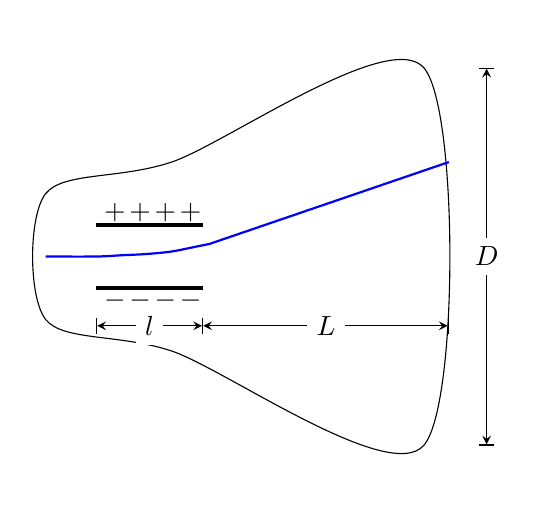
\begin{tikzpicture}[>=stealth, scale=0.8]
    \draw plot[smooth cycle] coordinates {(0, 1) (2, 1.5) (6, 3) (6, -3) (2, -1.5) (0, -1)};
    \draw[ultra thick] (0.8, 0.5) -- (2.5, 0.5);
    \draw[ultra thick] (0.8, -0.5) -- (2.5, -0.5);
    \foreach \x in {1.1, 1.5, 1.9, 2.3} {
      \node at (\x, 0.7) {$+$};
      \node at (\x, -0.7) {$-$};
    }
    \draw[thick, blue] plot[smooth] coordinates {(0, 0) (0.8, 0) (1.2, 0.02) (1.6, 0.04) (2, 0.08) (2.4, 0.16) (2.6, 0.2)} -- (6.4, 1.5);
    \draw[|<->|] (7, 3) -- node[fill=white] {$D$} (7, -3);
    \draw[|<->|] (0.8, -1.1) -- node[fill=white] {$l$} (2.5, -1.1);
    \draw[<->|] (2.5, -1.1) -- node[fill=white] {$L$} (6.4, -1.1);
  \end{tikzpicture}
  \end{center}

  Les plaques métalliques génèrent un champ électrique uniforme $\vec{E}$.
  Les dimensions du tube sont $l = \SI{2}{\centi\meter}$, $L =
  \SI{40}{\centi\meter}$ et $D = \SI{60}{\centi\meter}$.  Avant de passer entre
  les plaques du déflecteur, la vitesse des électrons est
  5\% de la vitesse de la lumière vers la droite.

  Déterminer la norme du champ électrique nécessaire pour que les électrons
  atteignent le haut de l'écran.


  Soit $v_x$ et $v_y$ les composantes horizontales et verticales de la vitesse
  des électrons à leur entrée entre les deux plaques.

  Pas de force dans la direction $x$ donc $v_x$ est constante: $v_x = 0.05c$.

  Le temps requis pour que les électrons traversent les plaques est
  \[
    t_l = \frac{l}{v_x}
  \]

  Pendant la traversée des plaques, les électrons sont soumis à une force
  constante vers le haut dont la grandeur est
  \[
    F = eE
  \]
  où $E$ est la grandeur du champ électrique. Par la deuxième loi de Newton
  \[
    a_y = \frac{eE}{m}.
  \]
  La composante verticale de la vitesse à la sortie des plaques est donc
  \[
    v_{yl} = \frac{eE t_l}{m} = \frac{eEl}{mv_x}
  \]
  Le déplacement vertical pendant le passage entre les plaques est
  \begin{eqnarray*}
    y_l &=& \frac{1}{2} a_y t_l^2 \\
    &=& \frac{1}{2} \frac{eE}{m} \frac{l^2}{v_x^2} \\
    &=& \frac{eEl^2}{2mv_x^2}
  \end{eqnarray*}
  Pour la partie après les plaques, il n'y a pas de force, donc vitesse
  constante.
  \[
    t_L = \frac{L}{v_x}
  \]
  et
  \begin{eqnarray*}
    y_L &=& v_{yl} t_L \\
    &=& \frac{eEl}{mv_x}\frac{L}{v_x} \\
    &=& \frac{eElL}{mv_x^2}.
  \end{eqnarray*}
  Pour atteindre le haut de l'écran, $y_L = D/2$ donc
  \begin{eqnarray*}
    \frac{D}{2} &=& \frac{eEl^2}{2mv_x^2} + \frac{eElL}{mv_x^2} \\
     &=& \frac{eEl}{mv_x^2} \left(\frac{l}{2} + L\right) \\
    E &=& \frac{Dmv_x^2}{2el (l/2 + L)} = \SI{46.7}{kN/C}
  \end{eqnarray*}


\sectionline


\section{Distributions de charge}

\marginpar{Tremblay \S 2.5}

\paragraph{Objectif}

\begin{enumerate}
  \item L'étudiant pourra calculer le champ électrique produit par une
    distribution de charge.
  \item L'étudiant comprendra qu'on peut diviser un objet étendu en petits
    morceau, considérer ces morceaux comme des particules, puis additionner les
    contributions de ces morceaux pour obtenir l'effet total.
  \item L'étudiant pourra utiliser le calcul intégral pour résoudre des
    problèmes de calcul de champ électrique.
\end{enumerate}


\subsection*{Exercice d'introduction aux distributions de charge}

\marginpar{10 minutes}

Chaque disque et l'anneau ont tous la même charge $Q$.
Classer les objets en ordre croissant de la grandeur du champ électrique au
point $P$.

\begin{center}
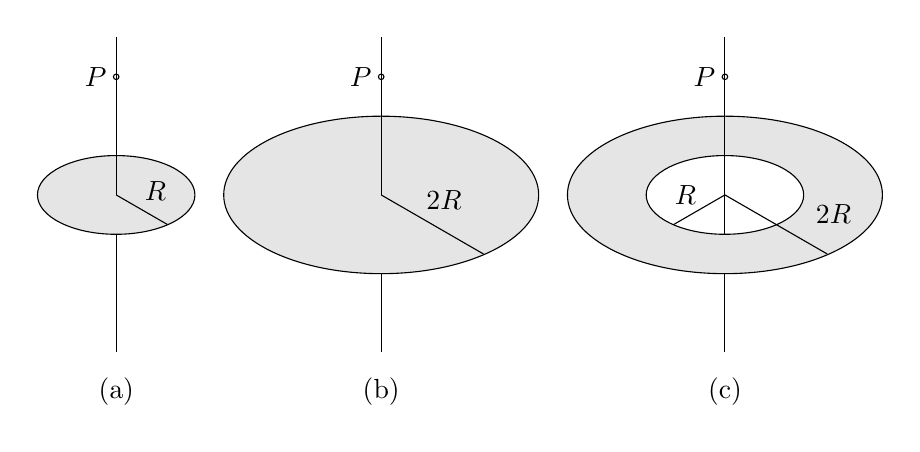
\begin{tikzpicture}
  \matrix[row sep=1em, column sep=1em] {
  \node at (0, -2.5) {(a)};
  \draw (0, 1.5) circle(1pt);
  \node[left] at (0, 1.5) {$P$};
  \draw (0,-2) -- (0,0);
  \draw[fill=black!10] (0,0) ellipse[x radius=1, y radius=0.5];
  \draw (0,0) -- (0,2);
  \draw (0,0) -- ++(-30:0.75);
  \node at (5:0.5) {$R$}; &
  \node at (0, -2.5) {(b)};
  \draw (0, 1.5) circle(1pt);
  \node[left] at (0, 1.5) {$P$};
  \draw (0,-2) -- (0,0);
  \draw[fill=black!10] (0,0) ellipse[x radius=2, y radius=1];
  \draw (0,0) -- (0,2);
  \draw (0,0) -- ++(-30:1.5);
  \node at (-05:0.8) {$2R$}; &
  \draw (0, 1.5) circle(1pt);
  \node[left] at (0, 1.5) {$P$};
  \node at (0, -2.5) {(c)};
  \draw (0,-2) -- (0,0);
  \draw[fill=black!10] (0,0) ellipse[x radius=2, y radius=1];
  \draw[fill=white] (0,0) ellipse[x radius=1, y radius=0.5];
  \draw (0,-0.5) -- (0,2);
  \draw (0,0) -- ++(-150:0.75);
  \node at (180:0.5) {$R$};
  \draw (0,0) -- ++(-30:1.5);
  \node at (-10:1.4) {$2R$};\\
  };
\end{tikzpicture}
\end{center}


\subsection*{Calcul de champ le long de l'axe d'une tige chargée}

\marginpar{20 minutes}

Comment peut-on calculer le champ électrique produit par un objet chargé qui
n'est pas ponctuel? La formule que nous avons vue ne s'applique pas.

Nous allons d'abord considérer une tige chargée (ou un fil) de longueur $L$
portant une charge totale $Q$ répartie uniformément dans la tige.

Un fil n'est pas une particule ponctuelle, mais on peut le subdiviser en petits
morceaux.

Un segment de longueur $\Delta x$ porte une fraction de la charge totale.

\paragraph{Question}: quelle fraction de la charge $Q$ est portée par un
segment de longueur $\Delta x$?

\begin{eqnarray*}
\Delta q &=& Q \frac{\Delta x}{L} \\
         &=& \frac{Q}{L} \Delta x
\end{eqnarray*}

On appelle le rapport $Q/L$ une  \textbf{densité linéique de charge}. On
utilise souvent le symbole $\lambda$ pour représenter une densité linéique
$$\lambda = \frac{Q}{L}$$
dans le cas d'une tige chargée uniformément.

Donc
$$\Delta q = \lambda \Delta x.$$

Si $\Delta x$ est suffisamment petit, on peut considérer ce morceau de fil
comme une charge ponctuelle. Le champ électrique généré par ce bout de fil est
donc
\begin{eqnarray*}
\Delta E_x &\approx& \frac{k \Delta q}{r^2} \\
           &\approx& \frac{k \Delta q}{(L + d - x)^2}
\end{eqnarray*}

Pour déterminer le champ électrique total, il suffit d'additionner les
contributions de toutes les parties du fil.

\begin{eqnarray*}
  E_x &\approx& \sum \frac{k \Delta q}{(L + d - x)^2}
\end{eqnarray*}

Tout ceci est approximatif parce que les parties de fil que nous avons
considérées ne sont pas réellement ponctuelles. Si nous voulons obtenir un
résultat exact, il faut que la longueur des segments de fils tende vers $0$.
Alors, la somme devient une intégrale

\begin{eqnarray*}
  E_x &=& \lim_{\Delta q \rightarrow 0}\sum \frac{k \Delta q}{(L + d - x)^2} \\
      &=& \int_{fil} \frac{k dq}{(L + d - x)^2} \\
      &=& \int_0^L \frac{k\lambda dx}{(L + d - x)^2} \\
      &=& \left[ \frac{k\lambda}{L + d - x} \right]_0^L \\
      &=& k\lambda \left( \frac{1}{L + d - L} - \frac{1}{L + d} \right) \\
      &=& k\lambda \left( \frac{1}{d} - \frac{1}{L + d} \right) \\
      &=& \frac{k\lambda L}{d(L+d)}
\end{eqnarray*}

Deux cas limites intéressants:

\begin{itemize}
  \item si $d \gg L$, on trouve $kQ/d^2$
  \item si $d \ll L$, on trouve $k\lambda / d$
\end{itemize}


\sectionline



\subsection*{Exercice dirigé --- Champ électrique au-dessus d'une tige chargée}

\paragraph{Partie 1 --- Symétrie et orientation du champ}
\marginpar{5 minutes}

En utilisant la symétrie de la situation, déterminer la direction dans la
laquelle le champ électrique doit être orienté au point $P$.

\begin{center}
  \includegraphics[scale=0.5]{02-champ-electrique/figures/champ-fil-3.pdf}
\end{center}


\textit{Solution. L'idée clé est que la composante horizontale du champ doit
  être nulle puisque les composantes horizontales des éléments de chaque côté
  du centre de la tige s'annulent deux à deux. La situation est illustrée
  ci-dessus.}

\paragraph{Partie 2 --- Champ produit par un élément de longueur}

À la lumière de la partie 1, trouver une expression pour la composante
verticale du champ électrique produit par un élément de longueur, i.e.: on
cherche une expression pour $dE_y$.

\begin{center}
  \begin{tikzpicture}
    \draw (-4, 0) -- (4, 0);
    \draw (-4, -0.1) -- (4, -0.1);
    \coordinate (P) at (0, 3);
    \coordinate (O) at (0, 0);
    \coordinate (l) at (-2, 0);
    \coordinate (r) at (2, 0);
    \node[anchor=west] (Pn) at (P) {$P$};
    \fill (P) circle(2pt);
    \draw[<->] (O) -- node[fill=white] {$D$} ($(P) - (0, 0.08)$);
    \fill ($(l) - (0.1, 0)$) rectangle ++(0.2, -0.1);
    \fill ($(r) + (0.1, 0)$) rectangle ++(-0.2, -0.1);
    \draw[dashed] (l) -- (P);
    \draw[dashed] (r) -- node[right] {$r$} (P);
    \draw[very thick,->] (P) -- ++({atan(3/2)}:1.5);
    \draw[very thick,->] (P) -- ++({180-atan(3/2)}:1.5);
    \draw ($(P) - (0, 0.5)$) arc (-90:{-atan(3/2}:0.5);
    \node at ($(P) + (0.2, -0.7)$) {$\theta$};
    \draw (0, -0.1) -- (0, -0.3) node[below] {$0$};
    \draw (r) -- ++(0, -0.3) node[below] {$x$};
    \draw[->] (-3.5, 1.5) -- (-2, 1.5) node[below] {$x$};
    \draw[->] (-3.5, 1.5) -- (-3.5, 3) node[left] {$y$};
  \end{tikzpicture}
\end{center}

  Un \textbf{élément de longueur} $d x$ produit un champ dont seule la
  composante verticale demeure (la composante horizontale étant annulée par
  celle d'un élément de longueur situé du côté opposé du fil.

  Pour trouver le champ électrique $dE_y$ produit, on fait l'approximation que
  l'élément de longueur est suffisamment petit pour qu'on puisse le considérer
  comme une charge ponctuelle. Le champ est donc

  $$d E_y = \frac{k d q}{r^2} \cos\theta.$$

  La charge est $dq = \lambda dx$ où $\lambda = Q / L$. La distance peut
  s'écrire

  $$d E_y = \frac{k \lambda dx}{r^2} \cos\theta.$$



\paragraph{Partie 3 --- Diminution du nombre de variables}

L'expression obtenue précédemment contient trois variables : $x$, $r$ et
$\theta$. Or, le fil est un objet à une dimension, il devrait donc être
possible d'exprimer l'élément de champ en terme d'une seule variable. Utiliser
la trigonométrie pour éliminer deux des trois variables.


On exprime tout en fonction de $\theta$. Il faut donc éliminer $x$ et $r$.

\begin{align*}
  \cos \theta &= \frac{D}{r} \\
           r  &= \frac{D}{\cos\theta}
\end{align*}

\begin{align*}
  \tan \theta &= \frac{x}{D} \\
           x  &= D\tan\theta \\
          dx  &= D\sec^2\theta d\theta
\end{align*}

Donc

  $$d E_y = \frac{k \lambda D\sec^2\theta d\theta}{D^2 / \cos^2\theta} \cos\theta.$$

qui se simplifie considérablement

  $$d E_y = \frac{k \lambda d\theta}{D} \cos\theta.$$



\paragraph{Partie 4 --- Application du principe de superposition}

Nous avons déterminé la composante verticale du champ produit par un élément de
longueur $dx$. Reste à déterminer la composante verticale du champ électrique
total au point $P$. Pour ce faire, nous n'avons qu'à intégrer l'expression que
nous avons obtenue sur toute la longueur de la tige. En faisant cela, nous
appliquons le principe de superposition.

\begin{align*}
  E_y &= \int_{\theta_1}^{\theta_2} \frac{k \lambda d\theta}{D} \cos\theta \\
      &= \frac{k \lambda}{D} \left[\sin\theta\right]_{\theta_1}^{\theta_2} \\
      &= \frac{k \lambda}{D} \left(\sin \theta_2 - \sin \theta_1 \right) \\
\end{align*}

Cette expression se simplifie en remarquant que
\begin{align*}
  \sin \theta_1 &= -\frac{L/2}{\sqrt{L^2/4 + D^2}} \\
  \sin \theta_2 &= \frac{L/2}{\sqrt{L^2/4 + D^2}} \\
\end{align*}

Donc
\[
  E_y = \frac{k \lambda}{D}\frac{L}{\sqrt{L^2/4 + D^2}}
\]

D'où
$$\vec{E} = \frac{k \lambda}{D}\frac{L}{\sqrt{L^2/4 + D^2}}\yhat$$


\paragraph{Partie 5 --- Vérification des cas extrêmes}

C'est toujours une bonne idée de vérifier les cas extrêmes pour s'assurer que
l'expression obtenue est cohérente dans ces cas. Qu'arrive-t-il si nous sommes
très loin de la tige ($D \gg L$)? Qu'arrive-t-il si nous sommes très proche
($D \ll L$)?

Loin:
\[
  E_y = \frac{k Q}{D^2}
\]

Proche: $\theta_1 = -\pi/2$ et $\theta_2 = \pi/2$ donc la différence des sinus
est $2$ et le champ est
\[
  E_y = \frac{2k\lambda}{D}
\]

